\chapter{Conclusions and Future Work}\label{chp:chp7}

\begin{flushright}
  {\em QUOTE GOES HERE }\\

\ \

\normalsize
{AUTHOR}  
\end{flushright}


\noindent{FIRST PARAGRAPH}

General features of profiles
-red scat wing
-absorption not necessarily blue flux biased
-peak may be central or blue-shifted
-double peaked emission lines may be seen due to absorption in central regions, but trough will be red-shifted

General limitations of modelling asymmetric line profiles
-complex/asymmetric geometries have significant effect on line profiles
-noisy
-most effective when can limit based on red wing, but still dependent on species
 
Broad results
-nonetheless obtain strong results that are broadly in agreement with SED fitting
-got evolution of SN~1987A in strong agreement with Gall 2014
-also got large masses at late times
-then the dust plot
-then wrap up lots of dust in sne and relate back to dust budget proble in the early universe - remind them what the point was!

\begin{figure}
\centering
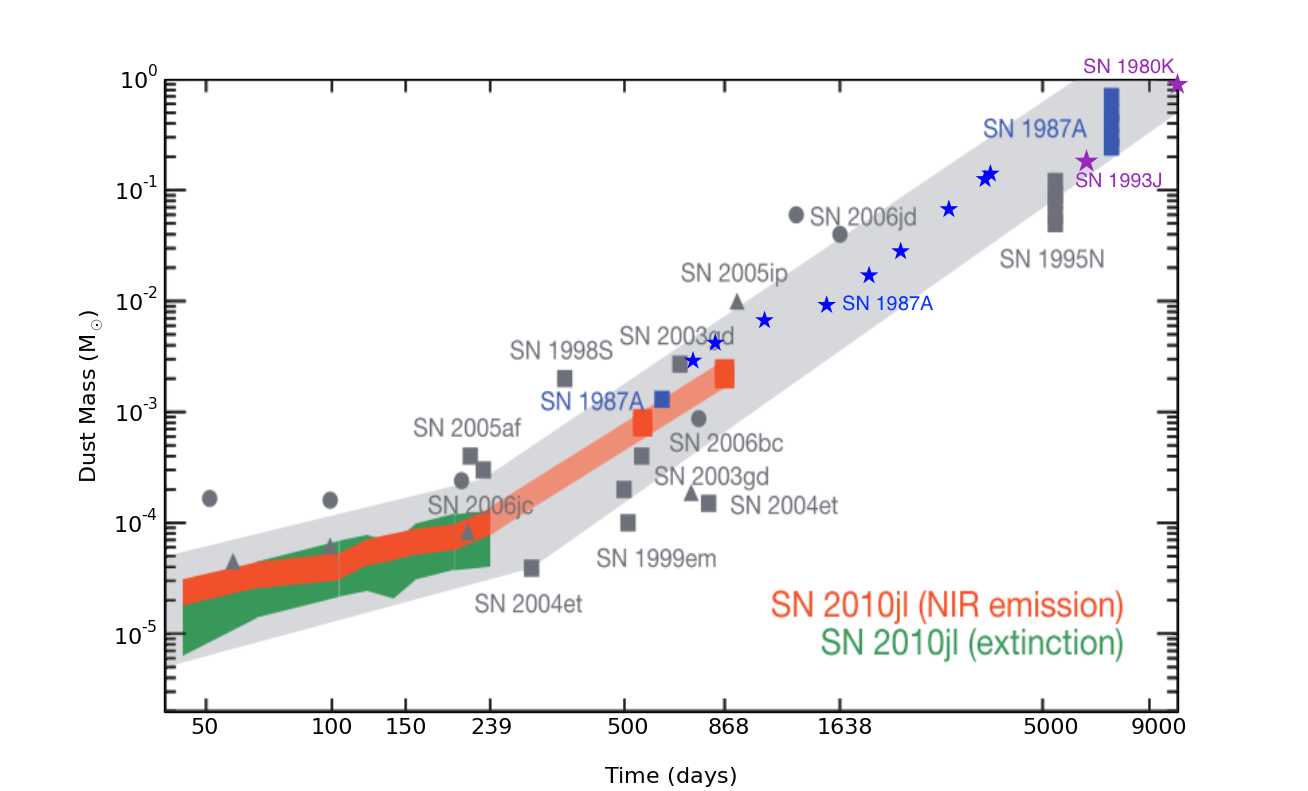
\includegraphics[scale=0.5,clip=true, trim=50 0 60 30]{chapters/chapter7/figs/final_dust_plot.png}
\caption{dust masses}
\label{shifted}
\end{figure}